% A LaTeX template for EXECUTIVE SUMMARY of the MSc Thesis submissions to
% Politecnico di Milano (PoliMi) - School of Industrial and Information Engineering
%
% P. F. Antonietti, S. Bonetti, A. Gruttadauria, G. Mescolini, A. Zingaro
% e-mail: template-tesi-ingind@polimi.it
%
% Last Revision: October 2021
%
% Copyright 2021 Politecnico di Milano, Italy. Inc. All rights reserved.

\documentclass[11pt,a4paper]{article}

%------------------------------------------------------------------------------
%	REQUIRED PACKAGES AND  CONFIGURATIONS
%------------------------------------------------------------------------------
% PACKAGES FOR TITLES
\usepackage{titlesec}
\usepackage{color}

% PACKAGES FOR LANGUAGE AND FONT
\usepackage[utf8]{inputenc}
\usepackage[english]{babel}
\usepackage[T1]{fontenc} % Font encoding

% PACKAGES FOR IMAGES
\usepackage{graphicx}
\graphicspath{{Images/}} % Path for images' folder
\usepackage{eso-pic} % For the background picture on the title page
\usepackage{subfig} % Numbered and caption subfigures using \subfloat
\usepackage{caption} % Coloured captions
\usepackage{transparent}

% STANDARD MATH PACKAGES
\usepackage{amsmath}
\usepackage{amsthm}
\usepackage{bm}
\usepackage[overload]{empheq}  % For braced-style systems of equations

% PACKAGES FOR TABLES
\usepackage{tabularx}
\usepackage{longtable} % tables that can span several pages
\usepackage{colortbl}

% PACKAGES FOR ALGORITHMS (PSEUDO-CODE)
\usepackage{algorithm}
\usepackage{algorithmic}

% PACKAGES FOR REFERENCES & BIBLIOGRAPHY
\usepackage[colorlinks=true,linkcolor=black,anchorcolor=black,citecolor=black,filecolor=black,menucolor=black,runcolor=black,urlcolor=black]{hyperref} % Adds clickable links at references
\usepackage{cleveref}
\usepackage[square, numbers, sort&compress]{natbib} % Square brackets, citing references with numbers, citations sorted by appearance in the text and compressed
\bibliographystyle{plain} % You may use a different style adapted to your field

% PACKAGES FOR THE APPENDIX
\usepackage{appendix}

% PACKAGES FOR ITEMIZE & ENUMERATES
\usepackage{enumitem}

% OTHER PACKAGES
\usepackage{amsthm,thmtools,xcolor} % Coloured "Theorem"
\usepackage{comment} % Comment part of code
\usepackage{fancyhdr} % Fancy headers and footers
\usepackage{lipsum} % Insert dummy text
\usepackage{tcolorbox} % Create coloured boxes (e.g. the one for the key-words)
\usepackage{stfloats} % Correct position of the tables
\usepackage{multirow}
\usepackage{multicol}
\usepackage{tikz}
\usetikzlibrary{positioning, arrows.meta}



%-------------------------------------------------------------------------
%	NEW COMMANDS DEFINED
%-------------------------------------------------------------------------
% EXAMPLES OF NEW COMMANDS -> here you see how to define new commands
\newcommand{\bea}{\begin{eqnarray}} % Shortcut for equation arrays
\newcommand{\eea}{\end{eqnarray}}
\newcommand{\e}[1]{\times 10^{#1}}  % Powers of 10 notation
\newcommand{\mathbbm}[1]{\text{\usefont{U}{bbm}{m}{n}#1}} % From mathbbm.sty
\newcommand{\pdev}[2]{\frac{\partial#1}{\partial#2}}
% NB: you can also override some existing commands with the keyword \renewcommand

%----------------------------------------------------------------------------
%	ADD YOUR PACKAGES (be careful of package interaction)
%----------------------------------------------------------------------------
\usepackage{amsfonts} 

%----------------------------------------------------------------------------
%	ADD YOUR DEFINITIONS AND COMMANDS (be careful of existing commands)
%----------------------------------------------------------------------------


% Do not change Configuration_files/config.tex file unless you really know what you are doing.
% This file ends the configuration procedures (e.g. customizing commands, definition of new commands)
% Set the geometric layout of the document
\usepackage{geometry}
\geometry{
  top=3cm,
  left = 2.0cm,
  right = 2.0cm,
  bottom=2cm,
  headheight= 2cm,
  headsep= 0cm,
}
\raggedbottom

% Create color bluePoli (-> manuale grafica coordinata:  https://www.polimi.it/fileadmin/user_upload/il_Politecnico/grafica-coordinata/2015_05_11_46xy_manuale_grafica_coordinata.pdf)
\definecolor{bluePoli}{cmyk}{0.4,0.1,0,0.4}

% Custom theorem environments
\declaretheoremstyle[
  headfont=\color{bluePoli}\normalfont\bfseries,
  bodyfont=\color{black}\normalfont\itshape,
]{colored}

\captionsetup[figure]{labelfont={color=bluePoli}} % Set colour of the captions
\captionsetup[table]{labelfont={color=bluePoli}} % Set colour of the captions
\captionsetup[algorithm]{labelfont={color=bluePoli}} % Set colour of the captions

\theoremstyle{colored}
\newtheorem{theorem}{Theorem}[section]
\newtheorem{proposition}{Proposition}[section]

% Enhances the features of the standard "table" and "tabular" environments.
\newcommand\T{\rule{0pt}{2.6ex}}
\newcommand\B{\rule[-1.2ex]{0pt}{0pt}}

% Algorithm description
\newcounter{algsubstate}
\renewcommand{\thealgsubstate}{\alph{algsubstate}}
\newenvironment{algsubstates}{
    \setcounter{algsubstate}{0}%
    \renewcommand{\STATE}{%
    \stepcounter{algsubstate}%
    \Statex {\small\thealgsubstate:}\space}
    }{}

% Custom theorem environment
\newcolumntype{L}[1]{>{\raggedright\let\newline\\\arraybackslash\hspace{0pt}}m{#1}}
\newcolumntype{C}[1]{>{\centering\let\newline\\\arraybackslash\hspace{0pt}}m{#1}}
\newcolumntype{R}[1]{>{\raggedleft\let\newline\\\arraybackslash\hspace{0pt}}m{#1}}

% Custom itemize environment
\setlist[itemize,1]{label=$\bullet$}
\setlist[itemize,2]{label=$\circ$}
\setlist[itemize,3]{label=$-$}
\setlist{nosep}

% Set separation of columns
\setlength{\columnsep}{30pt}

% Create command for background pic
\newcommand\BackgroundPic{% Adding background picture
	\put(230,358){
		\parbox[b][\paperheight]{\paperwidth}{%
			\vfill
			\centering
			\transparent{0.4}
			
\includegraphics[width=0.5\paperwidth]{raggiera_polimi.eps}%
			\vfill
}}}

% Set indentation
%\setlength\parindent{0pt}

% Custom title commands
\titleformat{\section}
{\color{bluePoli}\normalfont\Large\bfseries}
{\color{bluePoli}\thesection.}{1em}{}
\titlespacing*{\section}
{0pt}{2ex}{1ex}

\titleformat{\subsection}
{\color{bluePoli}\normalfont\large\bfseries}
{\color{bluePoli}\thesubsection.}{1em}{}
\titlespacing*{\subsection}
{0pt}{2ex}{1ex}

\titleformat{\subsubsection}
{\color{bluePoli}\normalfont\normalsize\bfseries}
{\color{bluePoli}\thesubsubsection.}{1em}{}
\titlespacing*{\subsubsection}
{0pt}{2ex}{1ex}

% Custom headers and footers
\pagestyle{fancy}
\fancyhf{}

\fancyfoot{}
\fancyfoot[C]{\thepage} % page
\renewcommand{\headrulewidth}{0mm} % headrule width
\renewcommand{\footrulewidth}{0mm} % footrule width

\makeatletter
\patchcmd{\headrule}{\hrule}{\color{black}\hrule}{}{} % headrule
\patchcmd{\footrule}{\hrule}{\color{black}\hrule}{}{} % footrule
\makeatother

% -> Create the header
\chead[C]{
\centering
\begin{tcolorbox}[arc=0pt, boxrule=0pt, colback=bluePoli!60, width=\textwidth, colupper=white]
    % \textbf{Homework 1} \hfill \textbf{\author}  
\end{tcolorbox}
}


% Insert here the info that will be displayed into your Title page
% -> title of your work
\renewcommand{\title}{Title}

% -> author name and surname
\renewcommand{\author}{Andrea Bonifacio, Sara Gazzoni}
% -> MSc course
\newcommand\norm[1]{\lVert#1\rVert}
\newcommand{\course}{Advanced Programming for Scientific Computing}
% -> advisor name and surname
\newcommand{\advisor}{Stefano Pagani}
% IF AND ONLY IF you need to modify the co-supervisors you also have to modify the file Configuration_files/title_page.tex (ONLY where it is marked)
\newcommand{\firstcoadvisor}{Mattia Corti} % insert if any otherwise comment
%\newcommand{\secondcoadvisor}{Name Surname} % insert if any otherwise comment
% -> academic year
\newcommand{\YEAR}{2022-2023}

%-------------------------------------------------------------------------
%	BEGIN OF YOUR DOCUMENT
%-------------------------------------------------------------------------
\begin{document}

%-----------------------------------------------------------------------------
% TITLE PAGE
%-----------------------------------------------------------------------------
% Do not change Configuration_files/TitlePage.tex (Modify it IF AND ONLY IF you need to add or delete the Co-advisors)
% This file creates the Title Page of the document
% DO NOT REMOVE SPACES BETWEEN LINES!

%\twocolumn[{\begin{@twocolumnfalse}

\AddToShipoutPicture*{\BackgroundPic}

\hspace{-0.6cm}
\includegraphics[width=0.6\textwidth]{logo_polimi_ing_indinf.eps}

\vspace{-1mm}
\fontsize{0.3cm}{0.5cm}\selectfont \bfseries \textsc{\color{bluePoli} Project Report}\\

\vspace{-0.2cm}
\Large{\textbf{\color{bluePoli}{\title}}}\\

\vspace{-0.2cm}
\fontsize{0.3cm}{0.5cm}\selectfont \bfseries \textsc{\color{bluePoli} \course}\\

\vspace{-0.2cm}
\fontsize{0.3cm}{0.5cm} \selectfont \bfseries Authors: \textsc{\textbf{\author}}\\

\vspace{-0.4cm}
\fontsize{0.3cm}{0.5cm}\selectfont \bfseries Advisors: \textsc{\textbf{\advisor}}\\

% if only ONE co-advisor is present:
\vspace{-0.4cm}
\fontsize{0.3cm}{0.5cm}\selectfont \bfseries Co-advisor: \textsc{\textbf{\firstcoadvisor}}\\
% if more than one co-advisors are present:
%\vspace{-0.4cm}
%\fontsize{0.3cm}{0.5cm}\selectfont \bfseries Co-advisors: \textsc{\textbf{\firstcoadvisor}}\textsc{\textbf{\secondcoadvisor}}\\

\vspace{-0.4cm}
\fontsize{0.3cm}{0.5cm}\selectfont \bfseries Academic year: \textsc{\textbf{\YEAR}}

\small \normalfont

\vspace{11pt}

\centerline{\rule{1.0\textwidth}{0.4pt}}

%\vspace{15pt}
%\end{@twocolumnfalse}}]

\thispagestyle{plain} % In order to not show the header in the first page


%%%%%%%%%%%%%%%%%%%%%%%%%%%%%%
%%     THESIS MAIN TEXT     %%
%%%%%%%%%%%%%%%%%%%%%%%%%%%%%%

%-----------------------------------------------------------------------------
% INTRODUCTION
%-----------------------------------------------------------------------------

\section{Introduction}
Full 3D blood flow models are important in the study of cardiovascular system since they allow one to extract detailed quantities of interest, but their actual implementation is limited due to their high computational cost. For this reason, reduced order models are widely used in this field because of their efficiency. An example is presented in \cite{Luca}, where a one-dimensional reduced order model is implemented to simulate the blood flow in the aorta using a graph neural network trained on three-dimensional simulations. In this work we propose a different application, where the graph neural network is used to approximate the solution of different problems. In particular, we consider the heat equation as test case, but the goal of the project is to show the potential extension of this approach to solve more difficult problems with complex geometries such as the simulations of proteins spreading in the neural system, which are at the basis of neurodegenerative diseases \cite{MattiaCorti}. The main part of this project is the implementation of a library for data generation used to train the graph neural network and the adaptation of the code [di Luca non so come citarlo] to make it suitable for our specific test case. In the following sections, we first present the problem formulation and a detailed description of the code developed, then we show the results obtained and a discussion of the possible further developments and extensions.

%-----------------------------------------------------------------------------
% Problem
%-----------------------------------------------------------------------------

\section{Problem overview}

% descrizione del problema generico Lu=F risolto con Fenics
We consider a general time-dependent variational problem of the form:
\[Lu=f\]
with \(L\) a linear operator, \(f\) a source term and \(u\) the solution. Given a specific geometry \(\Omega\) and using the finite element method implemented in FEniCS, we can solve this problem and obtain the solution \(u^{n}\) at each time step \(n\). From this, we can generate a graph that describes the geometry of the problem and the solution, storing some values of interest as features of the nodes and the edges.By solving the problem for different geometries and different values of the parameters(e.g. the diffusivity constant) we can generate a dataset that will be used to train the graph neural network. 

The graph neural network used in this project is the one presented in \cite{Luca}, which is an adaptation of the MeshGraphNet implementation \cite{MeshGraphNet}, which we modified to make it suitable for our test case and extendable to other problems.
The GNN is applied iteratively: at each time step it takes as input the system state \(\Theta^{n}\), which is the set of all the nodes and edges features at that time step, and it predicts an update for the state variables. The prediction is combined with the previous time step to estimate \(\Theta^{n+1}\). 
A forward step of the GNN is composed by three stages:
\begin{enumerate}
    \item Encode: a latent representation of the node and edge features is computed using a fully connected neural network.
    \item Process: the process stage is composed by L identical blocks, each of them is applied in sequence to the output of the previous blocs, updating the node and edge features. 
    \item Decode: using a fully connected neural network, the node features are transformed from the latent space to the output space. The output of the GNN is a vector containing the update of the state variables \(\delta\Theta^n\) at each node of the graph. 
\end{enumerate}
After this forward step, the state variables can be updated as \(\Theta^{n+1} = \Theta^{n} + \delta\Theta^{n}\).

% aggiungere tipo la loss 



\subsection{Test case: heat equation}
In this work, we consider the heat equation as test case. 
The mathematical formulation of the problem is the following:
\begin{equation}
    \begin{cases}
        \frac{\partial u }{\partial t} = k \Delta u \quad \text{in} \ \Omega \subset \mathbb{R}^2, \\
        \frac{\partial u}{\partial n} = h \quad \text{on} \ \partial \Omega_{inlet}, \\
        \frac{\partial u}{\partial n} = 0 \quad \text{on} \ \partial \Omega_{outlet} 
        \cup \partial \Omega_{walls}.
    \end{cases}
\end{equation}
where \(u\) is the temperature, \(k\) is the diffusivity constant, \(h\) is the Neumann condition at the inlet boundary. As domain \(\Omega\) we consider different geometries such as the one shown in Figure : the 2D mesh is composed of 4 trapezoids where the interface between them have different lengths.
% aggiungere figura di una mesh 

We generated 20 different mesh using gmsh. 
Then we solved the problem in FEniCS using Discontinuous Galerkin method and implicit Euler for time discretization, imposing as Neumann condition at inlet \(h = 2e^{-(t-2.5)^2}\).
From these solutions we generated a dataset of 277 graphs. 
Each graph has 5 nodes: an inlet node, an outlet node and 3 nodes in correspondence of the interfaces. 
As descriptor of the state of the system we consider the heat flux at each time step, which is computed as the integral of the normal derivative of the solution on the interface. The other node features are the thermal diffusivity \(k\), the interface length and the nodal type (inlet, outlet or branch node). 
As edge features we consider the area of the corresponding trapezoid and the distance between the nodes connected by the edge. 

% tabella con le varie features?

% training della GNN con i parametri

%-----------------------------------------------------------------------------
% Code
%-----------------------------------------------------------------------------

\section{Code}

% introduzione sulla struttura del nostro codice:
% mesh creation con gmsh -> potremmo creare una classe quindi magari 
% GenerateData.py: classi mesh loader, solver, data generator 
% GenerateGraph.py -> funzioni per generare i grafi 
% gNN

\subsection{Mesh creation}
\begin{figure}[H]
    \centering
    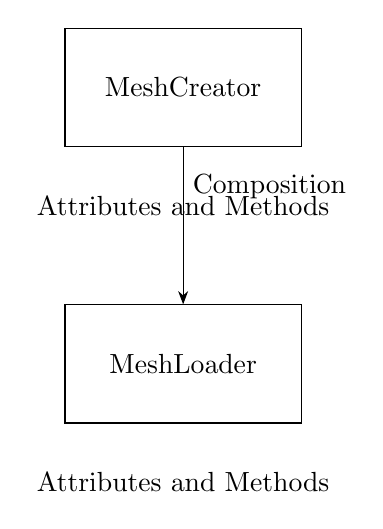
\begin{tikzpicture}[>=Stealth, node distance=2cm, class/.style={draw, rectangle, align=center, minimum width=3cm, minimum height=1.5cm}]

        % MeshCreator class
        \node[class] (MeshCreator) {MeshCreator};
        \node[class, below=of MeshCreator] (MeshLoader) {MeshLoader};

        % Arrows indicating composition
        \draw[->] (MeshCreator.south) -- ++(0,-0.5) -| (MeshLoader.north) node[midway, right] {Composition};

        % MeshLoader attributes and methods
        \node[below=0.5cm of MeshLoader] {Attributes and Methods};

        % MeshCreator attributes and methods
        \node[below=0.5cm of MeshCreator] {Attributes and Methods};

    \end{tikzpicture}
    \caption{Class Diagram for MeshCreator and MeshLoader}
\end{figure}

\subsection{Data generation}

\texttt{GenerateData.py} contains two abstract classes: \texttt{Solver} and \texttt{DataGenerator}. The first one is used to solve the variational problem, while the second one is designed to store all the quantities of interest whichwill be used to build the graphs. Each of these parent classes has two child classes: we start describing the solver one.
A diagram of the \texttt{Solver} class structure and methods is shown in Figure \ref{solver_class}.

\begin{figure}[H]
    \centering
    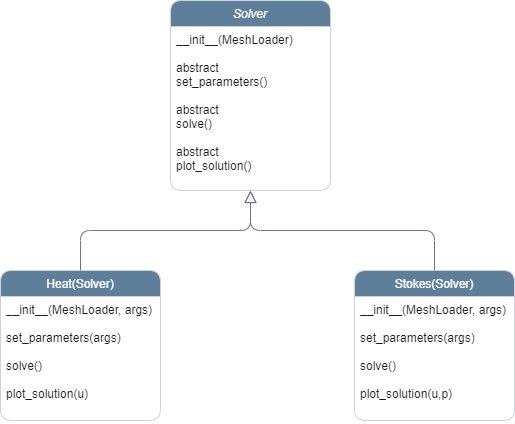
\includegraphics[width=0.5\textwidth]{Images/solver_class.png}
    \caption{Graph generated from the solution of the heat equation.}
    \label{solver_class}
\end{figure}

The abstract base class \texttt{Solver} contains the following methods:
\begin{itemize}
    \item \texttt{\_\_init\_\_(self,mesh)}: costructor that takes as input a \texttt{MeshLoader} object 
    \item \texttt{set\_parameters(self)}: abstract method
    \item \texttt{solve(self)}: abstract method
    \item \texttt{plot\_solution(self)}: abstract method
\end{itemize}

All the abstract method are overriden in the child classes \texttt{Heat} and \texttt{Stokes}. The choice of a parent abstract class for the solver is useful because it allows to use the same code for different problems, implementingchild classes that solve different equations, but with the same structure. 
We focus on the description of the \texttt{Heat} class, since it is the one used in the test case, but the \texttt{Stokes} class is implemented analogously.

The \texttt{Heat} class contains the following methods overriden from the parent class:
\begin{itemize}
    \item \texttt{\_\_init\_\_(self,mesh, V, k, f, u0, dt, T, g, doplot=False)}: constructor     which uses the \texttt{super()} function to inherit the base class constructor. The other problem parameters passed to the constructor are the function space, the diffusivity constant, the source term, the initial condition, the time step, the final step, the Neumann boundary condition at the inlet and a boolean variable to plot the solution at each time step. 
    \item \texttt{set\_parameters(self,V,k,f,u0,dt,T,g)}: function to set different problem parameters
    \item \texttt{solve(self)}: this method solves the Heat equation using Discontinuous Galerkin method and imposing a Neumann conditiona at the inlet boundary. The solution at each time step is stored in a list, as well as the time instants. 
    % decidere se si può mettere in degli numpy array 
    \item \texttt{plot\_solution(self,u)}: it takes as input the solution at a specific time step and it plots it.
\end{itemize}

The second abstract base class \texttt{DataGenerator} is schematized in Figure \ref{datagenerator_class}.

\begin{figure}[H]
    \centering
    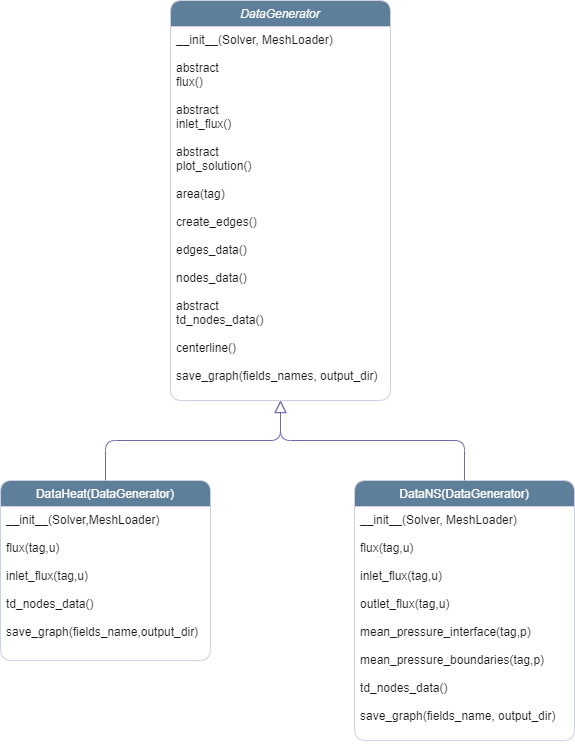
\includegraphics[width=0.5\textwidth]{Images/datagenerator_class.png}
    \caption{Graph generated from the solution of the heat equation.}
    \label{datagenerator_class}
\end{figure}

It contains the following methods:
\begin{itemize}
    \item \texttt{\_\_init\_\_(self,solver,mesh)}: constructor that takes as input a \texttt{Solver} object and a \texttt{MeshLoader} object
    \item \texttt{flux(self)}: abstract method 
    \item \texttt{inlet\_flux(self)}: abstract method
    \item \texttt{area(self,tag)}: concrete method that computes the area of the trapezoid corresponding to the tag passed as input 
    \item \texttt{nodes\_data(self)}: this function save as attribute of the object
    a dictionary containing the time independent nodes features. The keys of the dictionary
    are strings with the name of the features and the values are list (numpy array) containing 
    the values at each node.
    \item \texttt{td\_nodes\_data(self)}: abstract method
    \item \texttt{create\_edges(self)}: it stores as attributes of the object two lists (\texttt{self.edges1} and \texttt{self.edges2}) containing respectively the nodes ID of the source nodes of every edge and the node ID of the destination nodes.
    \item \texttt{edges\_data(self)}: it stores as attributes of the object a dictionary    containing the edge feature. The dictionary structure is analogous to the one of the node features.
    \item \texttt{centerline(self)}: this function computes the coordinates of the graph nodes, which are the coordinates of the centerline of the mesh at the interfaces. These coordinates are stored in a numpy array ?  
    \item \texttt{save\_graph(self, fields\_names, output\_dir)}: this method takes as input the name of the time dependent features of the graphs and the output directory where the graph has to be saves. It returns s dgl graph which is generated calling some functions defined in \texttt{generate\_graphs.py}, that will be described in the next section. 
\end{itemize}

As for the \texttt{Solver} class, the abstract methods are overriden in the two child classes \texttt{DataNS}
and \texttt{DataHeat}. The \texttt{DataHeat} class includes these methods:
\begin{itemize}
    \item \texttt{\_\_init\_\_(self,solver,mesh)}: constructor inherited from the parent class. 
    \item \texttt{flux(self,tag,u)}: method overriden from the parent class, it computes the heat flux of the solution \(u\) at the interface corresponding to the tag passed as input.
    \item \texttt{inlet\_flux(self,tag,u)}: method overriden from the parent class, it computes the heat flux at the inlet. The solution \(u\) and the tag of the inlet boundary are passe as input. 
    \item \texttt{td\_nodes\_data(self)}: methos overriden from the parent class, it stores as attribute of the object the time dependent nodes features in a dictionary. In this case the only time dependent feature is the heat flux: the dictionary has as key the time instant and as value a numpy array containg the heat flux at that time instant at each node.
    \item \texttt{save\_graphs}: method inherited from the parent class using the \texttt{super()} function, but the input \texttt{fields\_names} is a list containing only the string \texttt{'flux'}.
\end{itemize}

The \texttt{DataNS} is build analogously, with the only difference that the time dependent features are the flow rate and the pressure instead of the heat flux. In this case, the \texttt{flux} and \texttt{inlet\_flux} method computes the flow rate at the interfaces and at the inlet respectively. In addition, the class has a method \texttt{outlet\_flux} that computes the flow rate at the outlet and two other methods \texttt{mean\_pressure\_interface} and \texttt{mean\_pressure\_boundaries} that computes the mean pressure at the interfaces and at the inlet and outlet boundaries respectively.

\subsection{Graph generation}
In this section we describe the functions defined in \texttt{generate\_graphs.py} that are used to generate a dgl graph from the data obtained from the \texttt{DataGenerator} class. This file contains three functions: 
\begin{itemize}
    \item \texttt{generate\_graph(point\_data, points, edges\_data, edges1, edges2)}: this function takes as input a dictionary containing the time independent node features, a list (o numpy array) with the node coordinates, a dictionary containing the edge features and two lists containing the source and destination nodes of the edges. It return a dgl graph with the node and edge features stored as pytorch tensors.
    \item \texttt{add\_fields(graph, field, field\_name, offset=0)}: function to add a time dependent feature to the dgl graph. It take as input the dgl graph, a dictionary containing the field values at each time step, the name of the field and an offset with the number of time steps to skip. It returns the dgl graph with the new field added.
    \item \texttt{save\_graph(filename, output\_dir)}: function to save the dgl graph in a file in the output directory.
\end{itemize}

\subsection{Graph Neural Network}
The graph neural network used in this project is the one presented in \cite{Luca}, which is an adaptation of the MeshGraphNet implementation \cite{MeshGraphNet}, which we modified to make it suitable for our test case and extendable to other problems. The GNN is applied iteratively: at each time step it takes as input the system state \(\Theta^{n}\), which is the set of all the nodes and edges features at that time step, and it predicts an update for the state variables. The prediction is combined with the previous time step to estimate \(\Theta^{n+1}\). 

A forward step of the GNN is composed by three stages:
\begin{enumerate}
    \item Encode: a latent representation of the node and edge features is computed thanks to a first fully connected neural network.
    \item Process: the process stage is composed by \(L\) identical blocks, which update the node and edge features for \(L\) iterations. 
    \item Decode: using a fully connected neural network, the node features are transformed from the latent space to the output space. The output of the GNN is a vector containing the update of the state variables \(\delta\Theta^n\) at each node of the graph.
\end{enumerate}


%-----------------------------------------------------------------------------
% Results
%--- --------------------------------------------------------------------------

\section{Results}

%-----------------------------------------------------------------------------
% Further work
%-----------------------------------------------------------------------------

\section{Further work}

%---------------------------------------------------------------------------
%  BIBLIOGRAPHY
%---------------------------------------------------------------------------
\newpage
% Remember to insert here only the essential bibliography of your work
\bibliography{bibliography.bib} % automatically inserted and ordered with this command

\end{document}
